\section{TelcoGAN Model}
In this section, we introduce our TelcoGAN model for Telco missing data completion. The descriptions are separated into three parts. First, we describe the design of TelcoGAN model as well as the interaction of different components. Second, we give the details of relative coordinate space and explore the real-world relationship between connected cells and RSSI. Next, the designs of generator, discriminator and localizer is introduced respectively. Finally, we give TelcoGAN's training process.

\begin{figure}
  \centering
  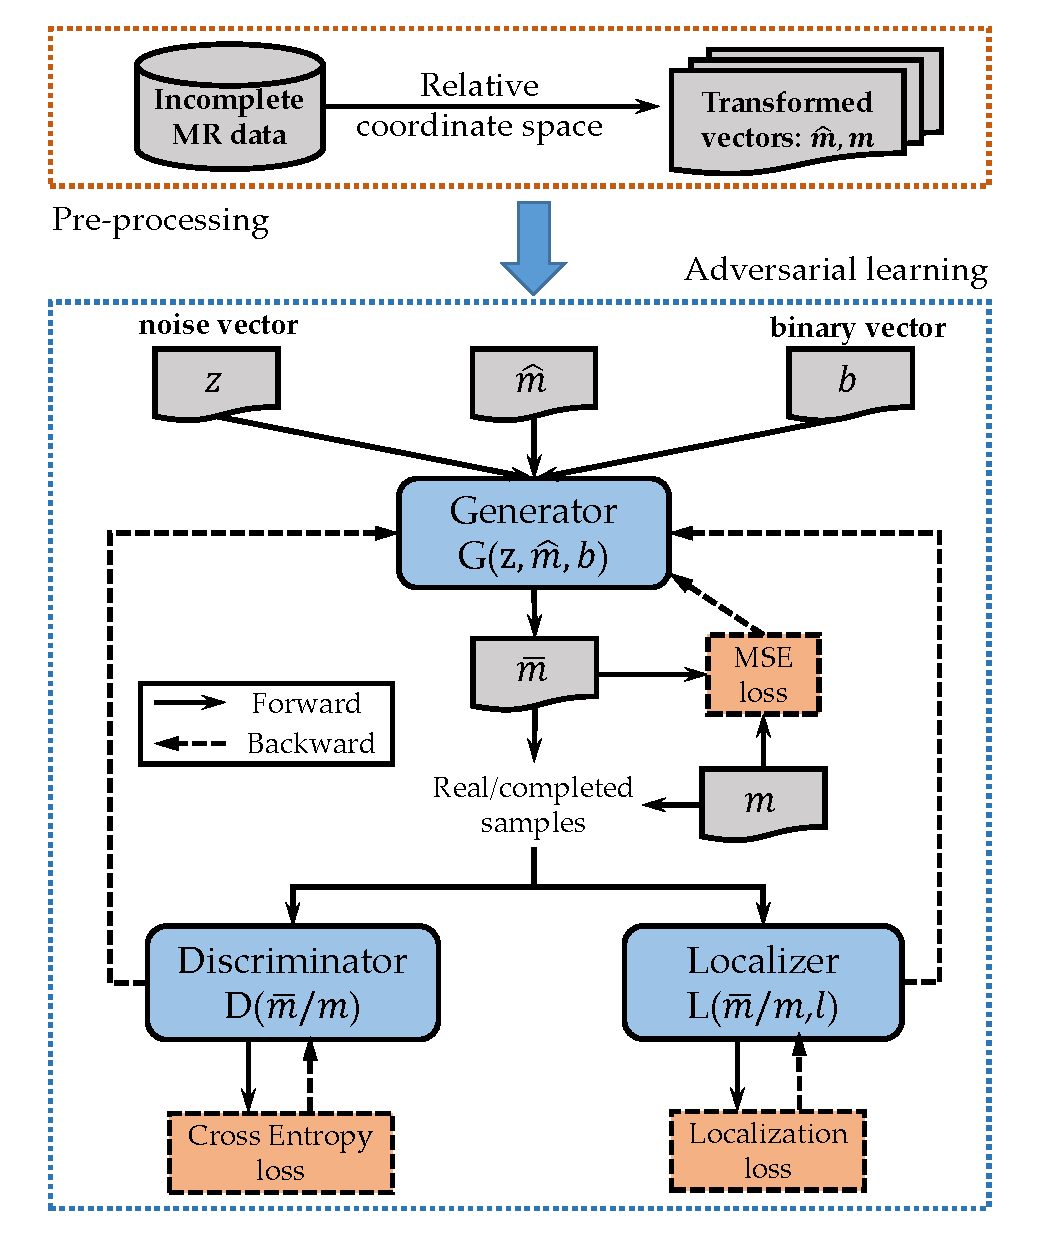
\includegraphics[width=9cm]{pics/framework.pdf}
  \caption{The framework of TelcoGAN}\label{fig:framework}
\end{figure}


\subsection{Overview of TelcoGAN}
The TelcoGAN model consists of pre-processing step and three basic components. The framework of TelcoGAN is illustrated as Fig. \ref{fig:framework}.

In the pre-processing step, due to sparse extensive cell locations in MR data, we propose to apply a serving-centric space. Then the sparse global coordinate-based distribution of MR data is transformed into a dense relative coordinate-based distribution. Thus TelcoGAN model can better capture the internal correlation of MR data. We assume the following notations: $m$ denotes the transformed complete MR matrix, $\hat{m}$ the input incomplete MR matrix, $\bar{m}$ the generated completed MR matrix and $l$ the associated position label.

The adversarial learning step consists of three interacting components described as follows:

(1) \textbf{Generator} $\bar{\textbf{m}}\sim$ G(\textbf{z},$\hat{\textbf{m}}$, \textbf{b}): The generator takes a random vector, an incomplete MR matrix and corresponding binary vector as input, and generates a completed MR matrix $\bar{\textbf{m}}$ that fools the discriminator as well as makes localizer produce accurate predictions.

(2) \textbf{Discriminator} D($\bar{\textbf{m}}/\textbf{m}$): The discriminator takes either a complete MR sample or a real MR sample as input, and gives each sample the probability over two categories (real/completed).

(3) \textbf{Localizer} L($\bar{\textbf{m}}/\textbf{m}$, $\textbf{l}$): The localizer takes a pair of MR sample and corresponding location label as input. It tries to predict the position of MR sample and minimize the localization loss.

The intuition of how our TelcoGAN model can generate high quality MR data for Telco localization is as follows. The generator tries to recover complete MR data samples based on observed variables to fool the discriminator; The discriminator distinguishes input data samples and computes probability distribution that the samples comes from real data or generated data; The localizer predicts locations of MR samples and produces a score for each sample that reflects its quality. During the adversarial game between the generator and the discriminator, the localizer can guide the optimization towards better data quality by utilizing available location labels. When the training reaches the optimality, the generator will have learnt the mapping from incomplete MR data to complete MR data.

We choose to implement these three components as neural networks. We will discuss their detailed structures for generating complete MR data in the following subsections.

\subsection{Serving-centric Space}
Here we construct a serving-centric space for MR data to better learn the internal relationship.

As seen in Table. \ref{tab:mr}, each MR record has a serving cell. According to Telco operations \cite{DBLP:conf/infocom/RayDM16}, the serving cell is selected from these nearby cells with good connection, which means close distance to mobile device. Thus a serving cell indicates a specific spatial domain. Given the total MR records with extensive global spatial domain, we group them as multiple local spatial domains by the serving cell. Then the whole city-scale area is divided into multiple small spatial domains.

Based on the division above, we propose a \emph{serving-centric space}, to transform the sparse global spatial distribution into a dense local one. In Fig. , a spatial domain is an area centered on the serving cell. Provided the cell tower database from Telco operators, we can obtain the GPS coordinate location of each cell. Based on the cell location data, we can do coordinate conversion as follows. Suppose the GPS coordinate (longitude, latitude) of the serving cell is $(x_0,y_0)$, those of the neighboring cells are $\{(x_i,y_i)\}$($1\leq i\leq 5$). Under the serving-centric space, the new coordinates are $(0,0)$ and $\{(x_i-x_0,y_i-y_0)\}$($1\leq i\leq 5$) for the serving cell and the neighboring cells respectively.

The \textbf{rational} behind serving-centric space is not difficult to understand: suppose normal cells and similar RF environment, in principle, the received signal strengths are only decided by the relative locations of connected cells and the MD. The serving-centric space offers advantages as: 1) reveal the true internal relationship of MR data and 2) knowledge learned from a domain can transfer to another domain and improve data quality.


\subsection{TelcoGAN Generator}
The goal here is to generate completed MR data by modelling the conditional probability distribution of missing components given the observed components. Note that to capture the uncertainty of the missing values \cite{buuren2010mice}, we choose to input random vectors for randomness.

We denote the input incomplete MR matrix as $\hat{m}=\{x', y', \hat{r}\}$, where $x'/y'$ is the relative latitude/longitude vector of connected cells, and $\hat{r}$ is the RSSI vector with missing values. We also denote the input random vector as $z$. To enable the randomness unified into the input MR matrix, we use the binary indicator vector $b$ as:

\begin{equation}\label{eq:b}
b_i=\left\{
\begin{aligned}
&0, &\text{if}\enspace\hat{r}_i=nan \\
&1, &\text{otherwise}
\end{aligned}
\right.
\end{equation}

so that $b$ indicates which positions of $\hat{r}$ are missing. 

Thus, the missing values of $\hat{r}$ is filled with $(1-b)\odot z$, where $\odot$ denotes element-wise multiplication. The input data matrix of generator G is computed as $\{x', y', \hat{r}+(1-b)\odot z\}$. The generator G can be formulated with:

\begin{eqnarray}
% \nonumber % Remove numbering (before each equation)
  \tilde{m} &=& G(z, \hat{m}, b) \\
  \bar{m}   &=& \tilde{r}\odot (1-b) + \hat{r}\odot b
\end{eqnarray}

To capture the internal relationship between observed components and missing components, we construct an encoder-decoder network as generator network. The encoder network consists of convolutional layers, and the decoder network consists of deconvolutional layers. The encoder network is used to extract features that reflects context of MR record such as location, environment and etc. Because the input incomplete MR matrix and output completed MR matrix have the same size, the deconvolutional layers of decoder network are used to restore information of MR record. We use convolution kernel with $3\times 3$ in convolutional layers to reduce the size of input data matrix.

\subsection{TelcoGAN Discriminator}
The TelcoGAN discriminator aims to differentiate completed MR records from the real ones by modelling the distribution of MR data.

The discriminator D takes either a completed MR record or a real MR record as input, and outputs the probability over two categories (real/completed). The D learns the probability of MR data $P(m)$ by full-convolution structure.

\subsection{TelcoGAN Localizer}
The TelcoGAN localizer is designed to exploit the available position labels in training phase. 

\subsection{TelcoGAN Training}
